\documentclass[a4paper,11pt,oneside]{article}

\usepackage[utf8]{inputenc}
\usepackage[T1]{fontenc}
\usepackage[english]{babel}
\usepackage{amssymb}
\usepackage{amsmath}
\usepackage{graphicx}
\usepackage{float}
\usepackage{hyperref}
\usepackage[dvipsnames]{xcolor}
\usepackage{listings}
\usepackage[top=2cm, bottom=2.5cm, right=2.5cm, left=2.5cm]{geometry}

\renewcommand{\familydefault}{\sfdefault}
\parindent0pt
\parskip6pt
\hypersetup{colorlinks=true,urlcolor=blue,linkcolor=blue}

\begin{document}

\title{Probability of having to wait longer in the shorter queue}
\author{Alexander Herzog\\\href{mailto:alexander.herzog@tu-clausthal.de}{\small\texttt{alexander.herzog@tu-clausthal.de}}}
\date{}

\maketitle

If there are several checkouts to choose from in a supermarket, for example, people tend to queue at the checkout with the shortest line in order to minimize their waiting time.

However, experience shows that this strategy is not always effective. Since the service times for individual customers are subject to random fluctuations (one customer has more in their shopping basket, another less; payment processes take different amounts of time), it can happen that the longer queue happens to have many orders that can be processed quickly, while the shorter queue has mostly orders that take more time. In this case, one may have to wait longer in the shorter queue than in the longer queue.

Mathematically, it can be shown that this situation occurs more frequently
\begin{itemize}
\item the more unpredictable the work orders from individual customers are,
\item the more customers there are in the queues and
\item the smaller the difference in the length of the queues is.
\end{itemize}

Conversely, if all work orders are equally complex, one is guaranteed to be served more quickly at the checkout with the shorter queue.



\section{Mathematical formulation of the problem}

To analytically calculate the probability of waiting longer in the shorter queue than in the longer one, we use the following designations:

\begin{itemize}
\item
We arrive at the checkout area of a supermarket. Two checkouts are open (and there is one cashier working at each open checkout, so two times $c=1$ applies).
\item
The service rate at both checkouts is $\mu>0$. The service times are exponentially distributed. There are therefore no structural differences between the checkouts in terms of service times. (Structural differences visible from the outside would be, for example, if one checkout is a “maximum 3 items” checkout or if one checkout is explicitly set up for cash payments only or card payments only.)
\item
When we arrive, there are $a\in\mathbb{N}$ people at the first checkout and $b\in\mathbb{N}$ at the second checkout. The number includes both customers waiting and customers currently being served.
\item
Let $a>b$, i.\,e., there are more people at the first checkout than at the second. Since there is no systematic difference in the service times at the two checkouts, it makes sense to favor the second checkout.
\end{itemize}

We are looking for the probability of having to wait longer at the second checkout than would have been the case at the first checkout, i.\,e., mathematically formulated:

$$
P(W_{(b)}>W_{(a)})
$$
(despite $b<a$).



\section{Exponential distribution}

The following section will focus on determining the distribution for the own service time depending on the choice of queue. The own service time is the sum of the remaining service time of the customer currently being served and the sum of the service times of all other customers ahead of oneself in the queue.

The service times of waiting customers (whose service has not yet begun) are subject to exponential distribution according to the above assumption. In order to calculate the convolution of the individual time durations, the distribution of the remaining service time of the customer currently being served has also to be determined.

The following holds for the cumulative distribution function $F(t)$ of the exponential distribution:
$$
P(X\le t)=F(t)=1-e^{-\mu t} \quad\text{für}\quad t\geq0.
$$
For the remaining service time of a customer who has already been served for $t_0\ge0$ time units, the following applies according to the definition of conditional probability:
\begin{eqnarray*}
P(X\le t+t_0|X\ge t_0)
&=&\frac{P(\{X\le t+t_0\}\cap \{X\ge t_0\})}{P(X\ge t_0)}
 = \frac{P(t_0\le X\le t+t_0)}{P(X\ge t_0)}\\
&=&\frac{F(t+t_0)-F(t_0)}{1-F(t_0)}\\
&=&\frac{(1-e^{-\mu(t+t_0)})-(1-e^{-\mu t_0})}{1-(1-e^{-\mu t_0})}
 = \frac{-e^{-\mu t}\cdot e^{-\mu t_0}+e^{-\mu t_0}}{e^{-\mu t_0}}\\
&=&1-e^{-\mu t}
 = F(t)=P(X\le t).
\end{eqnarray*}
This means that the probability that the remaining service time of a customer who has already been served for $t_0$ time units is less than or equal to $t$ is the same as the probability that the service time of a newly arriving customer is less than or equal to $t$. In other words, the remaining service time of a customer who has already been served for $t_0$ time units is also exponentially distributed with the same distribution parameter $\mu$. How long the customer has already been served therefore plays no role (if the exponential distribution is assumed for the service times) in determining their remaining service time. This property of the exponential distribution is also referred to as \emph{memorylessness}.



\section{Convolution of the exponential distribution}

We now know that our waiting time at a checkout where there are $n$ customers ahead of us ($n-1$ waiting and one being served) is composed of the sum of $n$ exponentially distributed random variables. We are therefore looking for the distribution of the sum of $n$ independent, exponentially distributed random variables $X_1,\ldots,X_n$.

The probability density function of the distribution, which is the sum of two distributions (with robability density functions $f$ and $g$), is denoted by $f*g$ and calculated as follows:
$$
(f*g)(x)=\int_{-\infty}^{\infty} f(x-y)g(y)\,dy.
$$
This process is called the \emph{convolution} of probability density functions. The probability density function of the distribution of one's own waiting time is therefore the $n$-fold convolution of the probability density function of the exponential distribution. The $n$-fold convolution of a probability density function $f$ with itself is denoted by $f^{*n}$.

By induction, it can be calculated that the $n$-fold convolution of the probability density functions of the exponential distribution with parameter $\mu$ yields the probability density functions of the Erlang distribution with parameters $n$ and $\mu$. The following applies to the probability density functions and the cumulative distribution function of the Erlang distribution:
\begin{eqnarray*}
f_{\mu,n}(t)&=&\frac{t^{n-1}e^{-\frac{t}{\mu}}}{\mu^n(n-1)!},\\
F_{\mu,n}(t)&=&1-e^{-\frac{t}{\mu}}\cdot\sum_{k=0}^{n-1}\frac{1}{k!}\left(\frac{t}{\mu}\right)^k \quad\text{für}\quad t\geq0.
\end{eqnarray*}

The probability of having to wait longer than $t\ge0$ seconds in a service system with $c=1$ operator and $n\in\mathbb{N}$ customers is therefore:

$$
P(W_{(n)}>t)=
1-P(W_{(n)}\le t)=
1-F_{\mu,n}(t)=
e^{-\mu t}\cdot\sum_{k=0}^{n-1}\frac{(\mu t)^k}{k!}.
$$



\section{Conditional distribution}

The quantity sought, $P(W_{(b)}>W_{(a)})$, is a conditional distribution: Normally, the question is how likely it is that the value of a random variable $X$ will be less than or greater than a fixed number $t$. Here, however, two random variables $W_{(a)}$ and $W_{(b)}$ are related. This probability can be calculated using the \emph{conditional distribution}:

\begin{eqnarray*}
P(W_{(b)}>W_{(a)})&=&
\int_{\mathbb{R}^+}P(W_{(b)}>W_{(a)}|W_{(a)}=t)\cdot f_{W_{(a)}}(t)~dt\\
~&=&
\int_{\mathbb{R}^+}P(W_{(b)}>t)\cdot f_{W_{(a)}}(t)~dt\\
~&=&
\int_{\mathbb{R}^+}
\left(e^{-\mu t}\cdot\sum_{k=0}^{b-1}\frac{(\mu t)^k}{k!}\right)\cdot\left(\frac{\mu^at^{a-1}e^{-\mu t}}{(a-1)!}\right)~dt\\
~&=&
\frac{\mu^{a-1}}{(a-1)!}\cdot\int_{\mathbb{R}^+}\sum_{k=0}^{b-1}\frac{(\mu t)^k}{k!}\cdot t^{a-1}\cdot\mu\cdot e^{-2\mu t}~dt\\
~&=&
\frac{1}{2}\cdot\frac{\mu^{a-1}}{(a-1)!}\cdot\int_{\mathbb{R}^+}\sum_{k=0}^{b-1}\frac{(\mu t)^k}{k!}\cdot t^{a-1}\cdot2\mu\cdot e^{-2\mu t}~dt\\
~&=&
\frac{1}{2}\cdot\frac{\mu^{a-1}}{(a-1)!}\cdot\sum_{k=0}^{b-1} \frac{\mu^k}{k!}\int_{\mathbb{R}^+}t^{a+k-1}\cdot2\mu\cdot e^{-2\mu t}~dt.
\end{eqnarray*}



\section{Moments of the exponential distribution}

We will now take a closer look at the expression
$$
\int_{\mathbb{R}^+}t^{a+k-1}\cdot2\mu\cdot e^{-2\mu t}~dt\;.
$$

\begin{itemize}
\item It was $a>b$ and $a,b\in\mathbb{N}$, i.\,e.\ $a\ge2$. Thus, $n:=a+k-1\in\mathbb{N}$ for all $k\in\mathbb{N}_0$.
\item Next, to the abbreviation $\tilde\mu:=2\mu$.
\end{itemize}

This allows us to write the above expression as:
$$
\int_{\mathbb{R}^+}t^{n}\cdot\tilde\mu\cdot e^{-\tilde\mu t}~dt.
$$
But that is precisely the $n$th moment of the exponential distribution with parameter $\tilde\mu$:
$$
\mathbf{E}[X_{\tilde\mu}^n]=
\int_{\mathbb{R}^+}t^{n}\cdot\tilde\mu\cdot e^{-\tilde\mu t}~dt=
\int_{\mathbb{R}^+}t^{n} f_{\tilde\mu}(t)~dt
$$
(with $f_{\tilde\mu}(t):=\tilde\mu\cdot e^{-\tilde\mu t}$). Induction can be used to show that the following applies to the moments of the exponential distribution with parameter $\tilde\mu$:
$$
\mathbf{E}[X_{\tilde\mu}^n]=\frac{n!}{\tilde\mu^n}.
$$
So here it is:
$$
\int_{\mathbb{R}^+}t^{a+k-1}\cdot2\mu\cdot e^{-2\mu t}~dt=
\mathbf{E}[X_{2\mu}^{a+k-1}]=\frac{(a+k-1)!}{(2\mu)^{a+k-1}}.
$$



\section{Final calculation of the probability sought}

Using the above considerations, the probability $P(W_{(b)}>W_{(a)})$ can now be calculated:

\begin{eqnarray*}
P(W_{(b)}>W_{(a)})&=&
\frac{1}{2}\cdot\frac{\mu^{a-1}}{(a-1)!}\cdot\sum_{k=0}^{b-1} \frac{\mu^k}{k!}\int_{\mathbb{R}^+}t^{a+k-1}\cdot2\mu\cdot e^{-2\mu t}~dt\\
~&=& \frac{1}{2}\cdot\frac{\mu^{a-1}}{(a-1)!}\cdot\sum_{k=0}^{b-1} \frac{\mu^k}{k!} \frac{(a+k-1)!}{(2\mu)^{a+k-1}}\\
~&=& \frac{1}{2}\cdot\frac{1}{(a-1)!}\cdot\sum_{k=0}^{b-1}\frac{1}{k!}\cdot\frac{(a+k-1)!}{2^{a+k-1}}\\
~&=& \left(\frac{1}{2}\right)^a\cdot\sum_{k=0}^{b-1}\frac{(a+k-1)!}{k!\cdot(a-1)!}\cdot\left(\frac{1}{2}\right)^k.
\end{eqnarray*}

With the definition of the binomial coefficient
$$
\binom{n}{k}:=\frac{n!}{k!\cdot(n-k)!}
$$
the final result follows:

\begin{eqnarray}
\nonumber
P(W_{(b)}>W_{(a)})&=&
\left(\frac{1}{2}\right)^a\cdot\sum_{k=0}^{b-1}\frac{(a+k-1)!}{k!\cdot(a-1)!}\cdot\left(\frac{1}{2}\right)^k\\
~&=&
\left(\frac{1}{2}\right)^a\cdot\sum_{k=0}^{b-1}\binom{a+k-1}{k}\cdot\left(\frac{1}{2}\right)^k.
\label{eq:PWbBiggerThanWa}
\end{eqnarray}




\section{Python implementation}

The result formula \eqref{eq:PWbBiggerThanWa} can be easily implemented in Python. The function \texttt{binom} from the module \texttt{scipy.special} is used to calculate the binomial coefficient. The function \texttt{PWbBiggerThanWa(a, b)} calculates the probability of having to wait longer at a checkout with $b$ customers than at a checkout with $a$ customers (with $a>b$ and assuming an exponential distribution for the service times):

\vskip0.5em
\begin{lstlisting}[inputencoding={utf8},frame=single]
from scipy.special import binom

def PWbBiggerThanWa(a, b):
    assert a > b, "a has to be bigger than b"
    return 0.5**a*sum([binom(a+k-1, k)*0.5**k for k in range(b)])
\end{lstlisting}
\vskip0.5em

If we vary $b$ (the length of the shorter queue) in the range from 1 to 25 and choose $a:=b+1$, $a:=b+2$ and $a:=b+3$, we obtain the graphs shown in Figure \ref{fig:PWbBiggerThanWa}.

\begin{figure}[H]
\centering
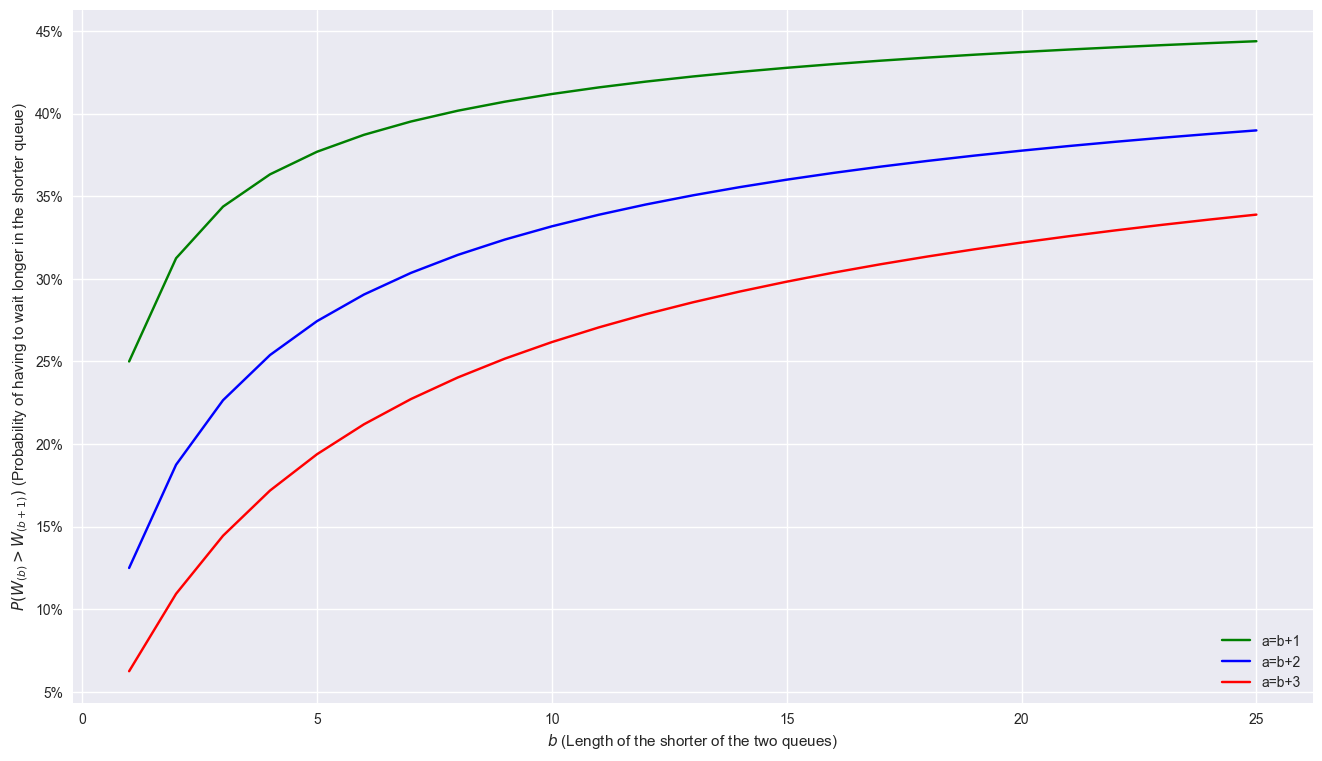
\includegraphics[width=0.99\textwidth]{ShorterQueue.png}
\caption{Probability of having to wait longer in the shorter queue}
\label{fig:PWbBiggerThanWa}
\end{figure}

It is clear to see that the probability of having to wait longer in the shorter queue (high $y$ values) increases the smaller the difference in the length of the queues is (green graph) and also the longer the two queues under consideration are overall (large $x$ values).

You can try out this behavior interactively on the following webpage:\\
\href{https://a-herzog.github.io/QueueCalc/?function=ShortestQueueValues}{a-herzog.github.io/QueueCalc/?function=ShortestQueueValues}

\end{document}
